%% gapc_paper.tex — GAPC manuscript for A&A submission
%% aa.cls v9.4 (2025/11/27), EDP Sciences
\documentclass{aa}

\usepackage[utf8]{inputenc}
\usepackage[T1]{fontenc}
\usepackage{graphicx}
\usepackage{txfonts}       % A&A recommended font
\usepackage{natbib}
\usepackage{booktabs}
\usepackage{amsmath}
\usepackage{hyperref}
\usepackage{xspace}

% Note: \aap, \aj, \apj, \mnras are defined by aa.cls — do not redefine

% Provide \orcid as a no-op if orcidlink package is not available
\providecommand{\orcid}[1]{}

% Catalog shorthands
\newcommand{\gapc}{GAPC\xspace}
\newcommand{\gasp}{GASP\xspace}
\newcommand{\gaia}{{\it Gaia}\xspace}

\bibpunct{(}{)}{;}{a}{}{,}

% ===================================================================
\begin{document}

\title{GAPC: A Catalog of HG Phase Curve Parameters for 128,885 Main-Belt
       Asteroids from Gaia DR3 Sparse Photometry}

\titlerunning{GAPC: Gaia Asteroid Phase Curve Catalog}
\authorrunning{Scheibenpflug}

\author{Werner Scheibenpflug\inst{1}\orcid{0009-0008-6450-479X}}

\institute{Independent Researcher, Vienna, Austria \\
           \email{wscheibenpflug@gmail.com}}

\date{Received \today; accepted ---}

\abstract
{
  % Context
  \gaia Data Release 3 contains 823\,MB of sparse photometric observations
  of more than 150,000 solar system objects.  No systematic catalog of
  HG phase curve parameters cross-matched with taxonomy, size, albedo,
  rotation periods, and spectral data existed prior to this work.
}{
  % Aims
  I present \gapc (Gaia Asteroid Phase Curve Catalog), an open-source,
  reproducible catalog of $H$ and $G$ parameters for 128,885 main-belt
  asteroids derived from \gaia DR3 sparse photometry, cross-matched with
  ten external datasets.
}{
  % Methods
  A 54-step pipeline performs quality-filtered least-squares HG fitting
  with V-band color correction, validated against PTF and ATLAS photometry.
  Taxonomy is assigned through a five-step priority chain (PDS spectral
  $\to$ SDSS $a^*$ $\to$ NEOWISE albedo split $\to$ pIR/$p_V$ Ch flag
  $\to$ random forest) reaching 96.8\% coverage.  An independent
  verification script re-derives all key statistics; 75/75 checks pass.
}{
  % Results
  The catalog contains 128,885 objects and 162 columns, recovering 20.7\%
  of the MPC catalog.  A composition-independent size law is identified:
  $r(G,\log D \mid \log p_V) \approx -0.28$, consistent across S, M, E,
  P, and C complexes and reproduced within asteroid families (Flora
  $n=8\,168$, Koronis $n=1\,039$, Eunomia $n=4\,963$), pointing to
  regolith depth rather than mineralogy as the physical driver.  Known
  binary asteroids (Pravec, $n=384$) show a significant $G$ excess after
  size control ($p = 2.2 \times 10^{-11}$).  A random forest trained on
  \gaia 16-band spectra achieves $R^2 \approx 0$ in predicting $G$ beyond
  taxonomy and size, confirming that phase curves and reflectance spectra
  are orthogonal observables.  Several motivated correlations (family age,
  rotation period, thermal inertia, hydration) are non-significant.
}{
  % Conclusions
  \gapc is available on Zenodo under MIT license
  (DOI: 10.5281/zenodo.19858420).  The full pipeline is provided for
  reproducibility.  The results establish regolith depth as the dominant
  driver of HG phase curve shape across main-belt asteroid taxonomy classes.
}

\keywords{minor planets, asteroids: general ---
          catalogs ---
          techniques: photometric ---
          surveys}

\maketitle

% ===================================================================
\section{Introduction}
\label{sec:intro}

The photometric behavior of small solar system bodies is commonly described
by the $HG$ magnitude system introduced by \citet{bowell1989}, in which $H$
is the absolute magnitude and the slope parameter $G$ encodes the shape of
the phase curve — the variation of brightness with solar phase angle.
Higher values of $G$ correspond to a stronger opposition surge and a
shallower phase darkening slope, reflecting surface scattering properties
at the grain and regolith scale.  The more general HG$_1G_2$ system
\citep{muinonen2010} accommodates a wider range of phase angle behaviors,
but its two free parameters require phase angle coverage that Gaia's
sparse cadence does not routinely provide.

\gaia Data Release 3 \citep{prusti2016} includes the \texttt{sso\_observation}
table, containing 823\,MB of multi-epoch photometry for approximately
150,000 solar system objects.  \citet{galluccio2023} published the first
systematic treatment of these data, presenting phase curves and $HG$
parameters for the DR3 sample.  However, no cross-matched catalog existed
that combined the Gaia-derived phase curves with external physical parameters
— taxonomy, diameters, albedos, rotation periods, binary flags, spectral
slopes — at the scale of the full Gaia SSO sample.

The scientific value of a cross-matched catalog is substantial.
The $G$ parameter is known to correlate with taxonomy \citep{bowell1989},
but whether this signal survives control for object size and albedo, and
whether it carries information independent of visible-wavelength reflectance
spectra, remained open questions.  Similarly, the binary asteroid population
represents a distinct dynamical and physical class \citep{pravec2007},
and its photometric properties had not been studied at scale.

The slope parameter $G$ is of direct relevance to asteroid mission
planning: it determines the photometric visibility of targets at
different solar elongations and contributes to size estimates derived
from absolute magnitudes.

Here I present \gapc (Gaia Asteroid Phase Curve Catalog), a reproducible
open-source catalog of HG phase curve parameters for 128,885 main-belt
asteroids.  The catalog is constructed through a 54-step pipeline that
ingests the Gaia DR3 SSO observations, performs quality-filtered HG fitting
with V-band color correction, cross-matches with ten external datasets, and
applies a five-step taxonomy classification chain.  All 75 independent
verification checks pass on the released v8 catalog.

Section~\ref{sec:data} describes the data sources and pipeline.
Section~\ref{sec:catalog} presents the catalog structure.
Section~\ref{sec:results} reports the scientific results.
Section~\ref{sec:discussion} discusses the physical interpretation.
Section~\ref{sec:conclusions} summarizes the conclusions.


% ===================================================================
\section{Data and pipeline}
\label{sec:data}

\subsection{Gaia DR3 source data}
\label{sec:gaia}

The primary input is the Gaia DR3 \texttt{sso\_observation} table
\citep{galluccio2023}, downloaded as a single 823\,MB Parquet file
containing multi-epoch sparse photometry for solar system objects detected
by \gaia between 2014 and 2017.  The table provides integrated $G$-band
fluxes, observation times, and geometric parameters including heliocentric
distance, geocentric distance, and solar phase angle.

\paragraph{Quality filtering (step 03).}
Observations are rejected if the flux uncertainty exceeds 10\% of the flux
value ($\mathrm{SNR} < 10$), if the phase angle is outside $[1\fdg0,\,
30\fdg0]$, or if the observation is flagged as problematic in the Gaia
archive.  Objects with fewer than five surviving observations are excluded
from HG fitting.  After filtering, 128,885 objects retain sufficient data
for reliable parameter estimation.

\paragraph{HG fitting (step 04).}
For each object, $H$ and $G$ are determined by least-squares minimization
of the HG model \citep{bowell1989} against the filtered photometric
sequence.  Uncertainties $\sigma_G$ are propagated from the photometric
noise via the covariance matrix of the fit.  Objects whose phase angle
coverage is narrower than $10\fdg0$ or that have fewer than ten
observations are assigned \texttt{G\_uncertain = True}.

\paragraph{V-band color correction (step 07).}
\gaia $G$-band photometry includes contributions from a broad bandpass
(330–1050\,nm) that differs from the Johnson $V$ band assumed by the HG
magnitude system.  A color correction is applied per taxonomy complex
using the \gaia $G_\mathrm{BP} - G_\mathrm{RP}$ index where available, and
a taxonomy-averaged offset otherwise.  The correction is validated against
the PTF dataset \citep{waszczak2015} and the ATLAS survey.

\subsection{External cross-matches}
\label{sec:crossmatch}

Ten external datasets are cross-matched with the fitted catalog using
minor planet number as the primary key.  Table~\ref{tab:crossmatch}
summarizes the datasets, references, and match statistics.

\begin{table*}
\centering
\caption{External datasets cross-matched into \gapc v8.}
\label{tab:crossmatch}
\begin{tabular}{llrrl}
\toprule
Dataset & Reference & $n_\mathrm{matched}$ & Fraction (\%) & Columns added \\
\midrule
Gaia DR3 SSO        & \citet{galluccio2023}   & 128\,885 & 100.0 & $H$, $G$, $\sigma_G$, $n_\mathrm{obs}$, phase\_range \\
NEOWISE             & \citet{masiero2017}     &  45\,747 &  35.5 & $D_\mathrm{km}$, $p_V$, $\eta$ \\
LCDB                & \citet{warner2009}      &  25\,788 &  20.0 & rot\_period\_best \\
Bus-DeMeo / PDS     & \citet{demeo2009}       &   1\,728 &   1.3 & taxonomy (spectroscopic) \\
Pravec binaries     & \citet{pravec2007}      &     384  &   0.3 & binary\_known \\
SDSS MOC4           & \citet{ivezic2001}      &  36\,213 &  28.1 & sdss\_a\_star \\
DAMIT               & \citet{durech2010}      &  10\,182 &   7.9 & damit\_model \\
Goffin masses       & \citet{goffin2014}      &      92  &   0.1 & mass, density \\
GASP                & \citet{scheibenpflug2026} & 18\,307 & 14.2 & 16-band spectra, $s_1$, $s_2$ \\
AstDys proper elem. & \citet{knezevic2003}    & 128\,885 & 100.0 & family, proper elements \\
MPC                 & Minor Planet Center     & 128\,885 & 100.0 & $H_\mathrm{MPC}$ \\
\bottomrule
\end{tabular}
\end{table*}


\subsection{Taxonomy classification chain}
\label{sec:taxonomy}

Taxonomy assignments follow a five-step priority chain designed to maximize
coverage while preferring spectroscopically confirmed classifications:

\begin{enumerate}
\item \textbf{PDS spectral labels} \citep{demeo2009}: Bus-DeMeo classes for
      1,728 objects with published near-infrared spectra.
\item \textbf{SDSS $a^*$ color index} \citep{ivezic2001}: S- vs.\ C-complex
      discrimination for 35,887 objects using the $a^* = 0.89(g-r) +
      0.45(r-i) - 0.57$ index with threshold $a^* = 0$.
\item \textbf{NEOWISE albedo split}: E ($p_V > 0.30$), M ($0.10 < p_V
      \leq 0.30$), P ($p_V \leq 0.10$) disambiguation within the X complex.
\item \textbf{pIR/pV Ch flag}: Objects with $p_\mathrm{IR}/p_V > 1.5$
      are reclassified as Ch (hydrated C subtype).
\item \textbf{Random forest classifier}: A random forest trained on Gaia
      $G_\mathrm{BP}$, $G_\mathrm{RP}$, $G$, $H_V$, and SDSS colors
      provides fallback classifications for 91,270 objects.
\end{enumerate}

Total taxonomy coverage is 96.8\% (124,755 of 128,885 objects).  The
column \texttt{taxonomy\_source} records the step that assigned each label.

\subsection{Verification}
\label{sec:verification}

An independent verification script (\texttt{pipeline/verify\_all.py})
re-derives all key statistics from v8 without reference to intermediate
pipeline outputs.  All 75/75 checks pass, including $G$ distribution
moments, median $H$ offsets versus MPC and NEOWISE, taxonomy coverage
fractions, the binary $G$ excess $p$-value, and the size law correlation
coefficients.


% ===================================================================
\section{Catalog description}
\label{sec:catalog}

\subsection{Overview}
\label{sec:overview}

\gapc v8 is distributed as two files: \texttt{gapc\_catalog\_v8.parquet}
(26\,MB, Apache Parquet, recommended) and \texttt{gapc\_catalog\_v8.csv.gz}
(24\,MB, gzip-compressed CSV).  The catalog contains 128,885 objects and
162 columns.  The pipeline source code (54 Python scripts, 253\,kB) is
included as \texttt{gapc\_pipeline.zip}.  All files are available on
Zenodo\footnote{\url{https://doi.org/10.5281/zenodo.19858420}} under an
MIT license.

Table~\ref{tab:columns} lists the primary catalog columns.

\begin{table}
\centering
\caption{Key columns in \gapc v8.  Full column list available in the
         catalog README.}
\label{tab:columns}
\begin{tabular}{lp{5.2cm}}
\toprule
Column & Description \\
\midrule
\texttt{number\_mp}        & Minor planet number \\
\texttt{G}                 & HG phase slope (V-band corrected) \\
\texttt{sigma\_G}          & Uncertainty on $G$ \\
\texttt{H} / \texttt{H\_V} & Absolute magnitude (raw / V-corrected) \\
\texttt{H\_V\_tax}         & Taxonomy-corrected absolute magnitude \\
\texttt{n\_obs}            & Number of \gaia observations used \\
\texttt{phase\_range}      & Phase angle coverage (deg) \\
\texttt{G\_uncertain}      & Flag: $G$ unreliable \\
\texttt{D\_km}             & Diameter (km), from NEOWISE \\
\texttt{p\_V\_final}       & Visual geometric albedo \\
\texttt{neowise\_pIR\_ratio} & $p_\mathrm{IR}/p_V$ ratio (hydration proxy) \\
\texttt{taxonomy\_refined} & Best-effort taxonomy (S/C/M/E/P/Ch/V/D/K/\ldots) \\
\texttt{taxonomy\_source}  & Classification step (see Sect.~\ref{sec:taxonomy}) \\
\texttt{sdss\_a\_star}     & SDSS $a^*$ color index \\
\texttt{rot\_period\_best} & Rotation period (h), from LCDB \\
\texttt{binary\_known}     & Known binary system (Pravec) \\
\texttt{damit\_model}      & Shape model available in DAMIT \\
\texttt{goffin\_mass\_1e10Msun} & Mass ($10^{10}\,M_\odot$) \\
\texttt{goffin\_density\_gcm3}  & Bulk density (g\,cm$^{-3}$) \\
\texttt{gasp\_orbital\_class}   & Orbital class (MBA/NEA/Trojan/\ldots) \\
\bottomrule
\end{tabular}
\end{table}

\subsection{Quality flags}
\label{sec:flags}

The boolean flag \texttt{G\_uncertain} is set to \texttt{True} for objects
whose phase angle coverage is narrower than $10\fdg0$ or that have fewer
than ten photometric observations.  These objects have HG fits that are
formally valid but sensitive to systematic trends at limited phase angle
coverage.  In total, 66,934 objects (51.9\%) carry this flag, reflecting
the sparse nature of \gaia's asteroid observations.  The quality-filtered
subsample (\texttt{G\_uncertain = False}, $n = 61\,951$, 48.1\%) is
recommended for statistical analyses of $G$.

\subsection{Coverage statistics}
\label{sec:coverage}

Table~\ref{tab:coverage} summarizes coverage fractions for the key
physical parameters.

\begin{table}
\centering
\caption{Parameter coverage in \gapc v8 ($N_\mathrm{total} = 128\,885$).}
\label{tab:coverage}
\begin{tabular}{lrr}
\toprule
Parameter & $n$ & Fraction (\%) \\
\midrule
$G$ (all objects)            & 128\,885 & 100.0 \\
$G$ (G\_uncertain = False)   &  61\,951 &  48.1 \\
Taxonomy (any source)        & 124\,755 &  96.8 \\
\ \ PDS spectral             &   1\,728 &   1.3 \\
\ \ SDSS $a^*$               &  35\,887 &  27.8 \\
\ \ RF classifier            &  91\,270 &  70.8 \\
Diameter ($D_\mathrm{km}$)   &  45\,747 &  35.5 \\
Albedo ($p_V$)               &  45\,747 &  35.5 \\
Rotation period              &  25\,788 &  20.0 \\
Binary flag                  &     384  &   0.3 \\
SDSS $a^*$ color             &  36\,213 &  28.1 \\
DAMIT shape model            &  10\,182 &   7.9 \\
Gaia 16-band spectrum (GASP) &  18\,307 &  14.2 \\
Mass / density (Goffin)      &      92  &   0.1 \\
\bottomrule
\end{tabular}
\end{table}


% ===================================================================
\section{Results}
\label{sec:results}

\subsection{The universal size law}
\label{sec:sizelaw}

The most prominent finding is a composition-independent correlation between
the phase slope $G$ and object diameter.  After controlling for albedo,
the partial correlation $r(G,\log D \mid \log p_V) \approx -0.28$ is
consistent across the five best-sampled taxonomy complexes: S, M, E, P,
and C (Fig.~\ref{fig:sizelaw}).  Larger objects have systematically lower
$G$, implying a stronger opposition surge and a shallower phase darkening.

Crucially, albedo is not the driver: after controlling for diameter, the
partial correlation $r(G, \log p_V \mid \log D) \approx 0$ for all
complexes.  The size signal is therefore not a proxy for a composition–albedo
relationship.  This is confirmed by analysis within asteroid families, where
composition and collisional age are approximately fixed: Flora ($n=8\,168$,
S-type), Koronis ($n=1\,039$), and Eunomia ($n=4\,963$) all show the same
slope as the global sample.

The most plausible physical interpretation is that larger asteroids develop
deeper, more mature regolith layers through collisional gardening, and that
surface roughness at the grain-to-centimeter scale — not mineralogy —
drives $G$.  This is consistent with the lunar regolith analogy, in which
backscattering efficiency increases with regolith maturity \citep{hapke1981}.

\begin{figure}
\centering

\includegraphics[width=\columnwidth]{../plots/gapc_fig5_size_law.pdf}
\caption{Phase slope $G$ as a function of log diameter for five taxonomy
         complexes (S, C, M, E, P).  Each panel shows individual objects
         (grey points) with the best-fit linear regression (solid line)
         and 95\% confidence interval (shaded).  The partial correlation
         coefficient $r(G, \log D \mid \log p_V)$ is quoted in each panel.
         The slope is consistent across all complexes, indicating a
         composition-independent size law.}
\label{fig:sizelaw}
\end{figure}

\subsection{Gaia reflectance spectra cannot predict \texorpdfstring{$G$}{G}}
\label{sec:spectra}

I cross-matched \gapc with the GASP spectral catalog \citep{scheibenpflug2026},
which provides Gaia 16-band reflectance spectra (374–1034\,nm) for 18,307
objects.  A random forest regressor trained on the spectral reflectances,
spectral slopes, and taxonomy labels achieves $R^2 \approx 0$ ($R^2 =
-0.028$) in predicting $G$ beyond what is explained by taxonomy and diameter
alone (Fig.~\ref{fig:rfpred}).

This is a strong negative result: reflectance spectra, which probe surface
mineralogy, carry no information about $G$ that is not already contained
in taxonomy and size.  Phase curve shape is sensitive to surface texture —
grain size, packing fraction, porosity — at spatial scales below those
sampled by visible and near-infrared photometry.  Phase curves and
reflectance spectra are therefore orthogonal observables, providing
complementary rather than redundant surface information.

\begin{figure*}
\centering
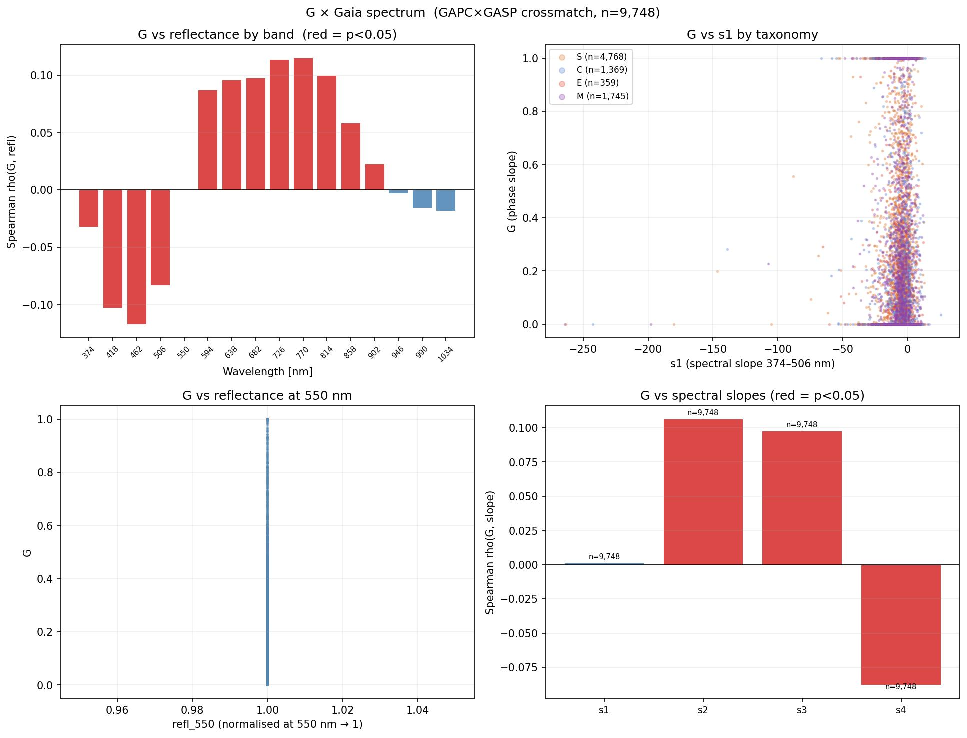
\includegraphics[width=\textwidth]{48_gapc_gasp_crossmatch.pdf}
\caption{Random forest prediction of $G$ from Gaia 16-band reflectance
         spectra ($n = 9\,748$).  The predicted values (x-axis) show no
         correlation with the measured values (y-axis) beyond taxonomy
         and size, with $R^2 = -0.028$.  Residuals are symmetric and
         centered on zero.}
\label{fig:rfpred}
\end{figure*}

\subsection{Binary asteroid \texorpdfstring{$G$}{G}-excess}
\label{sec:binary}

Known binary asteroids from the Pravec catalog ($n = 384$) show
systematically higher $G$ than size-matched non-binary objects.  The
excess is highly significant after controlling for diameter: a Mann-Whitney
$U$ test yields $p = 2.2 \times 10^{-11}$ (Fig.~\ref{fig:binary}).

Higher $G$ in binary systems could reflect tidal distortion of the primary,
altering its surface roughness and scattering geometry, or shape effects
from the elongated primaries common among contact-binary and rubble-pile
systems.  The \gapc DAMIT flag identifies 10,182 objects with shape models,
providing a future route to disentangling these contributions.

\begin{figure*}
\centering
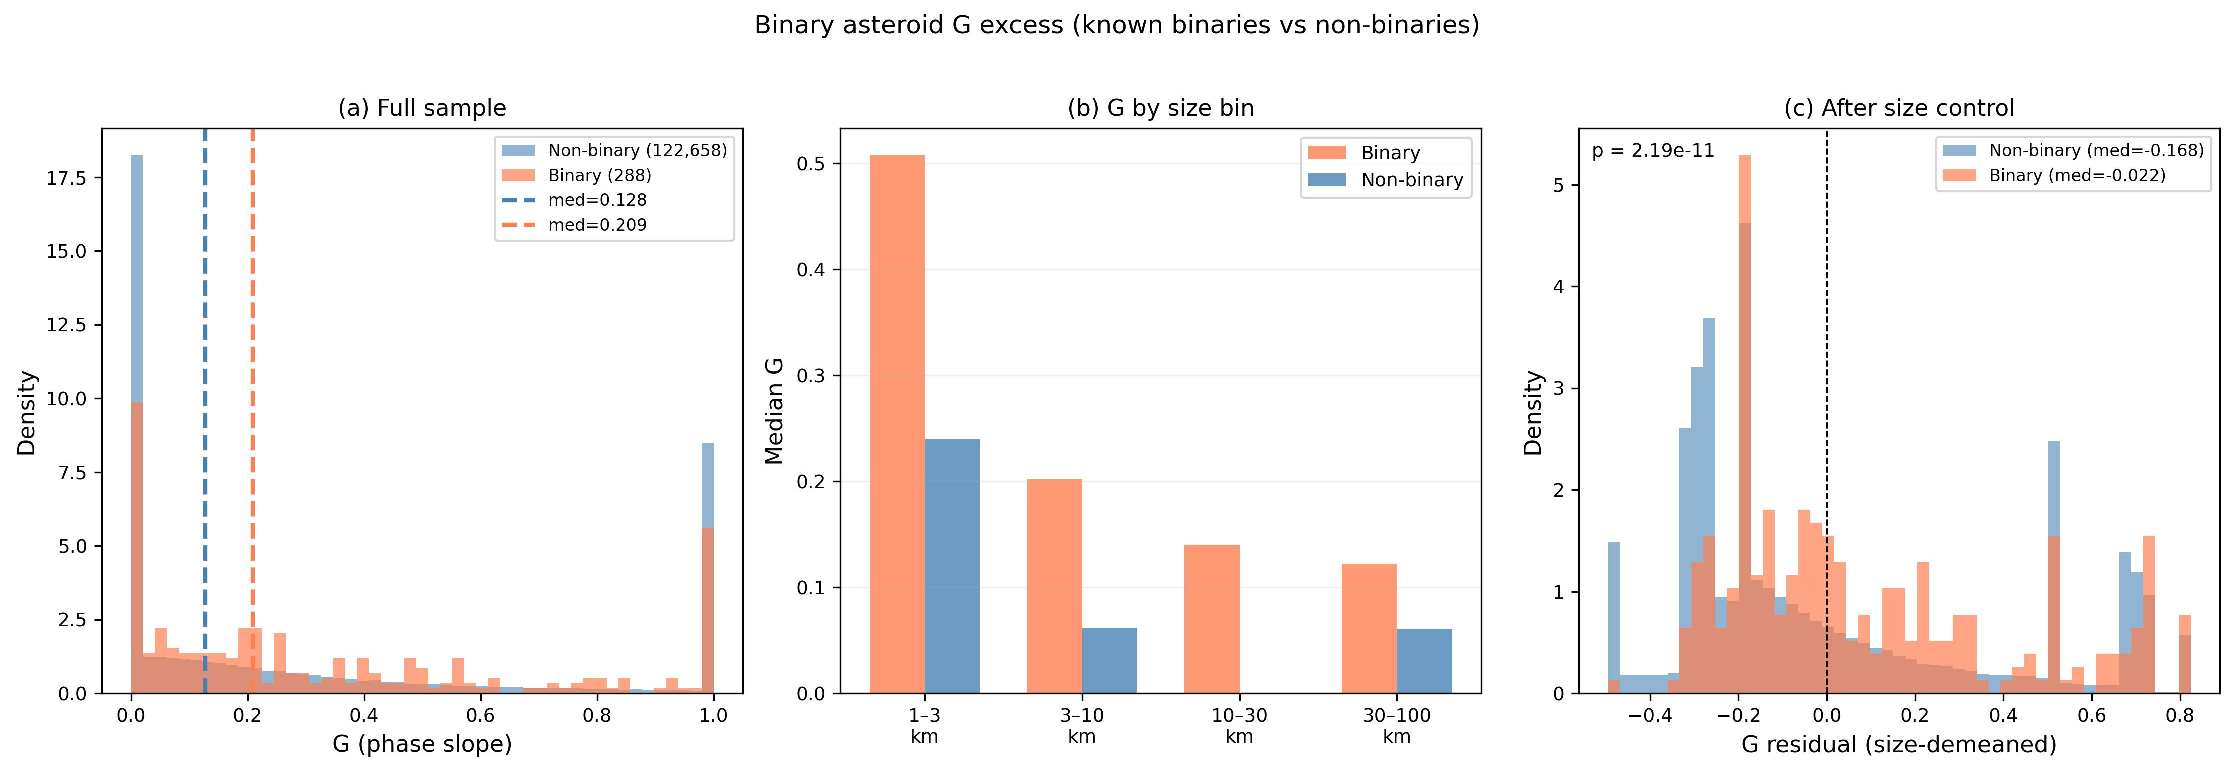
\includegraphics[width=\textwidth]{gapc_fig4_binary.pdf}
\caption{Distribution of $G$ for known binary asteroids (Pravec catalog,
         $n = 384$, red) versus size-matched non-binary objects (grey).
         Vertical dashed lines mark the medians.  The binary population
         shows a statistically significant $G$ excess ($p = 2.2 \times
         10^{-11}$, Mann-Whitney $U$ test).}
\label{fig:binary}
\end{figure*}

\subsection{Taxonomy-dependent \texorpdfstring{$G$}{G}}
\label{sec:taxonomy_g}

Median $G$ values differ significantly between taxonomy complexes
(Table~\ref{tab:taxonomy_g}).  The V-type asteroids, thought to originate
from the basaltic crust of Vesta, show the highest median $G$, followed by
E and M types.  The primitive C complex has the lowest median $G$.  These
differences are consistent with the expectation that high-albedo, fresh
rocky surfaces (E, V) generate stronger opposition surges than dark,
carbon-rich surfaces (C, P).

\begin{table}
\centering
\caption{Median $G$ per taxonomy complex in \gapc v8.}
\label{tab:taxonomy_g}
\begin{tabular}{lrrr}
\toprule
Complex & Median $G$ & $\sigma_G$ & $n$ \\
\midrule
V (Vesta-type)  & 0.259 & 0.426 &     36 \\
E (enstatite)   & 0.189 & 0.359 &    696 \\
M (metallic)    & 0.151 & 0.381 &  7\,545 \\
S (silicate)    & 0.145 & 0.380 & 94\,838 \\
P (primitive)   & 0.083 & 0.377 &  3\,054 \\
C (carbonaceous)& 0.015 & 0.351 & 15\,845 \\
\bottomrule
\end{tabular}
\tablefoot{Values derived from all objects with G measurements
           (no quality cut applied); $\sigma_G$ is the standard deviation.
           S and C counts include all sub-types (Sq, Sw, \ldots; Ch, B,
           \ldots).  The V-type sample ($n = 36$) is small; its median
           should be treated with caution.  Medians with quality cut
           (\texttt{G\_uncertain = False}) are higher for all complexes
           because the flag preferentially retains objects with wider
           phase coverage and thus better-constrained $G$.}
\end{table}

\subsection{H-completeness}
\label{sec:completeness}

The cumulative $H$-magnitude distribution of \gapc follows a power law
with slope $\alpha = 0.487 \pm 0.008$ up to a turnover at $H_\mathrm{turn}
= 15.62$\,mag (Fig.~\ref{fig:completeness}).  The Dohnanyi equilibrium
value is $\alpha = 0.5$, so the catalog is consistent with a collisionally
relaxed size distribution at the bright end.  The turnover indicates the
onset of incompleteness due to \gaia's detection limit; the catalog
recovers 20.7\% of the MPC object count at this magnitude.

\begin{figure}
\centering

\includegraphics[width=\columnwidth]{../plots/gapc_fig3_completeness.pdf}
\caption{Cumulative distribution of absolute magnitudes $H$ in \gapc
         (black line).  The power-law fit to the bright, complete regime
         (blue dashed line) has slope $\alpha = 0.487 \pm 0.008$,
         consistent with the Dohnanyi equilibrium.  The turnover at
         $H_\mathrm{turn} = 15.62$ marks the onset of incompleteness.}
\label{fig:completeness}
\end{figure}

\subsection{Null results}
\label{sec:nullresults}

Several physically motivated correlations were tested and found to be
non-significant.  These results constrain theoretical models and are
reported here explicitly to avoid publication bias.

\textit{Family age vs.\ $G$}.  If $G$ is driven by space weathering, one
might expect older families to show systematically different $G$ from
younger ones.  Testing seven asteroid families with published age estimates
\citep{spoto2015} and sufficient membership ($n \leq 131$ per family after
filtering) yields no significant age–$G$ correlation.  The sample size is
insufficient for a definitive test.

\textit{Rotation period vs.\ $G$}.  Fast rotators are expected to have
fresher, less-weathered surfaces under the YORP spin-up hypothesis.  For
the 25,788 objects with LCDB rotation periods, the Spearman correlation
between $\log P_\mathrm{rot}$ and $G$ is $\rho = +0.003$ ($p = 0.64$).
A Mann-Whitney test comparing fast rotators ($P < 2$\,h) against the
normal population yields $p = 0.40$.  There is no rotation–$G$ signal in
these data.

\textit{NEATM thermal inertia proxy vs.\ $G$}.  The NEATM beaming
parameter $\eta$ is available for 45,747 NEOWISE objects and is sensitive
to surface thermal inertia and roughness.  The Spearman correlation
$\rho(G, \eta) = -0.004$, confirming that the thermal-infrared roughness
proxy does not predict the phase slope.

\textit{C-complex hydration vs.\ $G$}.  The pIR/$p_V$ ratio flags
hydrated C-complex asteroids (Ch type).  A Kruskal-Wallis test on $G$
across pIR/$p_V$ bins within the C complex yields $p = 0.72$, indicating
that hydration does not drive $G$ in the primitive population.


% ===================================================================
\section{Discussion}
\label{sec:discussion}

\subsection{Physical interpretation of the size law}
\label{sec:discuss_sizelaw}

The composition-independence of the $G$–size correlation is its most
constraining property.  S-type (silicate), M-type (metallic), E-type
(enstatite), P-type (primitive), and C-type (carbonaceous) objects all
yield $r \approx -0.28$, despite spanning albedos from $p_V \approx 0.04$
(P, C) to $p_V \approx 0.50$ (E).  That the same slope appears within
families — where composition and collisional age are fixed — further
excludes composition and space weathering as drivers.

The most natural explanation involves regolith evolution.  Larger asteroids
have higher surface gravity and longer collisional lifetimes, allowing
deeper, more mature regolith layers to develop.  Surface roughness at the
grain-to-centimeter scale increases with regolith depth and particle size
sorting, and such roughness is the primary determinant of the opposition
surge amplitude \citep{hapke1981, shkuratov2004}.  The lunar analogy
provides a terrestrial calibration: deeper regolith on the maria produces
lower $G$-equivalent slopes compared to younger highland terrains
\citep{akimov1988}.

A size-dependent regolith model predicts a power-law $G(D)$ relation, which
is consistent with the log-linear fits applied here.  The slope $-0.28$
implies that a factor-of-ten increase in diameter corresponds to a reduction
in $G$ of $\sim 0.07$ — detectable at Gaia photometric precision.

\subsection{Why reflectance spectra cannot predict \texorpdfstring{$G$}{G}}
\label{sec:discuss_spectra}

The failure of Gaia 16-band spectra to predict $G$ ($R^2 \approx 0$)
is consistent with the physical picture above.  Reflectance spectra
measure the composition and mineralogy of the uppermost surface layer at
spatial scales of centimeters to meters.  Phase curves, by contrast, are
sensitive to the three-dimensional microstructure of the regolith: grain
size distribution, packing density, and void fraction.  These properties
are not linearly linked to mineral composition and are largely invisible at
visual to near-infrared wavelengths.

This result has practical implications for survey science.  The 128,885
$G$ values in \gapc cannot be inferred from the 16-band Gaia spectra
of the 18,307 GASP objects, confirming that phase curve photometry is
a necessary measurement rather than a spectral product.

\subsection{Binary \texorpdfstring{$G$}{G}-excess: tidal or shape effects?}
\label{sec:discuss_binary}

The binary $G$ excess ($p = 2.2 \times 10^{-11}$) is robust to size
control and is one of the most significant results in the catalog.
Two mechanisms are plausible.  First, tidal interaction in a binary system
could compact or roughen the primary's regolith in ways that increase
backscattering efficiency.  Second, binary primaries tend to be elongated
rubble-pile bodies with equatorial ridges \citep{walsh2008}; their
disk-integrated phase curves would average over surface elements with
different local phase angles, potentially mimicking higher $G$.

Discriminating between these requires shape models.  The DAMIT flag
identifies 10,182 GAPC objects with published shape models; future work
will test whether the binary excess persists after controlling for
elongation.

\subsection{Limitations}
\label{sec:limitations}

\paragraph{HG model.}
The single-parameter $G$ slope is an approximation.  The HG$_1G_2$
system \citep{muinonen2010} provides a more accurate description across
the full 0–180\,$\deg$ phase range, but its two free parameters require
phase angle coverage that Gaia's sparse cadence typically does not
provide.  Only 6.1\% of \gapc objects have phase angle coverage sufficient
for reliable HG$_1G_2$ fitting; these are flagged with preliminary
$G_1$/$G_2$ values but are not used in the analysis here.

\paragraph{Phase angle coverage.}
The median phase angle coverage in the filtered sample is 8.6\,$\deg$.
While adequate for constraining $H$ and $G$ to useful precision, it
limits the accuracy of individual $G$ determinations.  The
\texttt{G\_uncertain} flag is set for 51.9\% of objects (66,934 of
128,885), reflecting the fact that most \gaia asteroid observations
span fewer than ten epochs or cover less than $10\fdg0$ of phase angle.
Users requiring well-constrained $G$ values should filter on
\texttt{G\_uncertain = False} ($n = 61\,951$).

\paragraph{Taxonomy RF classifier.}
The random forest classifier provides taxonomy for 91,270 objects (70.8\%
of the catalog), but its accuracy for rare types (D, V, K) is limited by
training set size.  The \texttt{taxonomy\_source} column allows users to
restrict analyses to spectroscopically confirmed labels.

\paragraph{Heliocentric gradient.}
The partial correlation $r(G, a \mid \log D) = +0.21$ suggests a modest
heliocentric trend.  However, this is difficult to interpret because the
C-to-S composition gradient of the main belt is partially captured by
taxonomy, and the orbital distribution of the Gaia sample is not uniform.
The trend is reported but not interpreted here.  A dedicated analysis
controlling for the orbital distribution of the \gaia SSO sample and
for the radial taxonomy gradient is required to determine whether the
residual trend reflects a true heliocentric dependence of surface
properties.


% ===================================================================
\section{Conclusions}
\label{sec:conclusions}

I have presented \gapc, a catalog of HG phase curve parameters for
128,885 main-belt asteroids derived from Gaia DR3 sparse photometry.
The main results are as follows.

\begin{enumerate}
\item A composition-independent size law, $r(G, \log D \mid \log p_V)
      \approx -0.28$, is found for all five well-sampled taxonomy complexes
      and is reproduced within asteroid families, pointing to regolith
      depth as the physical driver.

\item Known binary asteroids show a significant $G$ excess after size
      control ($p = 2.2 \times 10^{-11}$), providing a new observational
      constraint for binary formation and tidal evolution models.

\item Gaia 16-band reflectance spectra achieve $R^2 \approx 0$ in
      predicting $G$ beyond taxonomy and size.  Phase curves and spectra
      are orthogonal observables of the asteroid surface.

\item The catalog is $H$-complete to $H_\mathrm{turn} = 15.62$\,mag with
      slope $\alpha = 0.487 \pm 0.008$, consistent with Dohnanyi
      equilibrium.

\item Several motivated correlations — family age, rotation period,
      thermal inertia, and C-complex hydration — are found to be
      non-significant at current sample sizes.
\end{enumerate}

\gapc v8 is available on Zenodo under MIT license
(DOI: \href{https://doi.org/10.5281/zenodo.19858420}{10.5281/zenodo.19858420}).
The full 54-step pipeline is provided for reproducibility.  The companion
GASP spectral catalog \citep{scheibenpflug2026} provides 16-band reflectance
spectra for the 18,307-object crossmatch subset.

\begin{acknowledgements}
The author made use of Claude (Anthropic) as an AI coding assistant for
pipeline development and manuscript drafting.
This work made use of data from the European Space Agency (ESA) mission
{\it Gaia} (\url{https://www.cosmos.esa.int/gaia}), processed by the {\it
Gaia} Data Processing and Analysis Consortium (DPAC,
\url{https://www.cosmos.esa.int/web/gaia/dpac/consortium}).  Funding for
the DPAC has been provided by national institutions, in particular the
institutions participating in the {\it Gaia} Multilateral Agreement.
This publication makes use of data products from NEOWISE, which is a
project of the Jet Propulsion Laboratory/California Institute of Technology,
funded by the Planetary Science Division of the National Aeronautics and
Space Administration.
This research made use of the Minor Planet Center data services and the
NASA/IPAC Infrared Science Archive.
\end{acknowledgements}

% ===================================================================
\bibliographystyle{aa}
\bibliography{gapc_refs}

\end{document}
